% !TEX root = ../Yan Hao--Dissertation.tex

\chapter{Questions on the Central Level}
Fiscal federalism is one typical form of fiscal decentralized structure. One consensus among economist and public administrative researchers is that decentralized fiscal structure is obviously more efficient in public goods and services supplying especially in those large and complex country with multiple level of administrative institutions. Hayek \cite{hayek2009use} states that the local government has significant advantages in knowing the information and supply proper kinds and amounts of public goods and services. Hayek's points is the starting points of the research in the advantage of fiscal federalism. Stiliger \cite{stigler1998tenable} followed Hayek's understanding and analyzed the necessity of intermediate and local government especially the necessity of protect the funding ability of those subnational governments. Tiebout \cite{tiebout1956pure} proved theoretically that voting on feat mechanism could promise the matching between public goods supply and needs. Besides, by introducing the competition rule of local governments into public area, Tiebout also proved that the decentralized structure is a promising tool in improving the administrative efficiency. Tiebout's theory seems get supported by the actual data showed in Table \ref*{Table 2.1}, which potentially reflects the difference of tax burden preference of different states. So for the following part, I'll only talk about the evaluation of decentralized fiscal structure, to be more specific, fiscal federalism.


  % Table generated by Excel2LaTeX from sheet 'Sheet1'
\begin{table}[H]
    \centering
    \caption{Effective Tax Revenue in America}
      \begin{tabular}{p{9.43em}lll}
      \toprule
      State & \multicolumn{1}{p{8.145em}}{State and Local Taxes (\$ billions)} & \multicolumn{1}{p{7.43em}}{Personal Income (\$ billions)} & \multicolumn{1}{p{9.93em}}{Effective Tax Rate} \\
      \midrule
      New York & \multicolumn{1}{c}{177.8} & \multicolumn{1}{c}{1,281.10} & \multicolumn{1}{c}{13.90\%} \\
      District of Columbia & \multicolumn{1}{c}{7.5} & \multicolumn{1}{c}{55.5} & \multicolumn{1}{c}{13.40\%} \\
      North Dakota & \multicolumn{1}{c}{5} & \multicolumn{1}{c}{39.5} & \multicolumn{1}{c}{12.70\%} \\
      Hawaii & \multicolumn{1}{c}{9.5} & \multicolumn{1}{c}{75.4} & \multicolumn{1}{c}{12.60\%} \\
      Vermont & \multicolumn{1}{c}{3.8} & \multicolumn{1}{c}{32.6} & \multicolumn{1}{c}{11.70\%} \\
      \midrule
      United States Total & \multicolumn{1}{c}{1,652.80} & \multicolumn{1}{c}{16,820.30} & \multicolumn{1}{c}{9.80\%} \\
      \midrule
      Alabama & \multicolumn{1}{c}{16.4} & \multicolumn{1}{c}{198.9} & \multicolumn{1}{c}{8.30\%} \\
      Oklahoma & \multicolumn{1}{c}{13.9} & \multicolumn{1}{c}{174.4} & \multicolumn{1}{c}{8.00\%} \\
      \midrule
      \multicolumn{4}{p{34.935em}}{\textit{Source:U.S. Census Bureau Dataset}} \\
      \end{tabular}%
    \label{Table 2.1}%
  \end{table}%
  
  
\section{How to Evaluate the Fiscal Federalism System}  
Even within the topic of fiscal federalism, the fiscal federalism structures in different countries have different content and features, needless to say, they show different impact in public goods and services supplying. Like I mentioned in Chapter 1, it's hard and nearly impossible to find a perfect stick yard criterion to compare fiscal federalism in different countries. I'll try to explain and get a comprehensive way to evaluate fiscal federalism. Literature about fiscal federalism can be roughly divided into two groups. First-generation theory of fiscal federalism concentrate on the fiscal structure itself, focusing on the efficiency of federalism in collecting revenue and offering responsibilities, and whether the revenue-responsibility combination perform well in public goods supply. Coming to second-generation theory of fiscal federalism, scholars get interested in the effect of fiscal federalism on other area such as the effect on economic development.

\subsection{First-Generation Theory of Fiscal Federalism}


One popular aspect to estimate if the  fiscal structure is reasonable is to evaluate the fiscal structure economically. In another word, to estimate if the combination of funding and responsibilities meet Pareto efficiency, which happens when resources are so allocated that it is not possible to make anyone better off without making someone else worse off \cite{pareto2014manual}. This is also the most common understanding wildly accepted by both economic and public administrative researcher.  Under economic view, three directions are helpful in estimating the fiscal structure, including externality, information complexity and incentive compatibility. Firstly, about externality, an ideal setting is to initialize the externality as much as possible for both positive and negative externality.Oates' \cite{oates1972fiscal} work on fiscal federalism is a milestone for modern fiscal federalism research, one principle he mentioned in his work is that government and the residents living in the jurisdiction should pay for their negative externality and get paid for positive externality.Olson \cite{olson1993dictatorship} states that the "free rider" issue could be overcome by making the jurisdiction and the  beneficiary area identical, besides, the equilibrium under this setting could make marginal cost equal to marginal benefits. The externality evaluation is obviously an efficiency consideration. 

Secondly, information complexity in administration process is also a important consideration in evaluating the fiscal federalism structure. Except for the earlier job represented by Hayek and Tiebout, Bsley et al \cite{2003Centralized} set up a political economy model to simulate the decision making process in a democratic country, in their model they introduced insensitivity of central government into their model and emphasized the advantage of local government in public goods supplying. Besides, the information communication is mutual. For one,local governments know local residents' needs better, besides, local governments' behavior could be better perceived by local residents. Dethier \cite{martinez2003fiscal} mentioned that the decentralized structure of fiscal federalism put the local government under supervision. Based on Dethier's idea and Tiebout's voting on feet framework, Baicker \cite{baicker2005spillover} set up a horizontal competition structure, he introduced multiple local governments and states that under yardstick competition framework, decentralized fiscal structure will help local residents get a direct evaluation about  local governments' efficiency in public goods supply, thus help them easier to "vote on feet". Local governments should get pushed by this information transparency.

Finally, a good fiscal structure should have incentive compatibility. Incentive compatibility is a game theory analysis tool introduced by Leonid Hurwicz \cite{hurwicz1973design} wildly used by business management area at first. A mechanism is called incentive-compatible (IC) if every participant can achieve the best outcome to themselves just by acting according to their true preferences. Incentive compatibility was introduced into public administration and public economics area and became an important criterion to evaluate the quality of fiscal federalism. Local governments could be motivated to supply proper amount and quantity public goods with efficiency under proper fiscal federalism setting. Eckstein \cite{eckstein1958water} points out that the proper combination between funding resource and responsibilities could be a great motivation for any kinds of organizations. Under Eckstin's setting, at least in democratic country, working hard with efficiency in public goods supplying is an weakly dominate strategy since that will attract more residents and increase more public funding resource. Another clue is that for most of the scholars, when they  investigate the related topic and talk about governmental fiscal behavior, while the central government's goal is hard to define, by default they just assume the local government's target is to maximize the local fiscal revenue(Baretti, Bucovetsky,Dahlby,Jha) \cite{baretti2002tax,bucovetsky2006efficiency,dahlby2011marginal,jha2000tax}. 

The main theme of the first-generation theory of fiscal federalism is to approve the positive effect of this decentralized structure, confirm the positive effect in public goods supplying. The main investigation is to evaluate the role of fiscal federalism in the public goods efficiency. Most of literature in this period is theoretical investigation. 

\subsection{Second-Generation Theory of Fiscal Federalism}
When it comes to the second-generation theories, scholars do not merely stare at the efficiency of fiscal federalism in public goods supplying. For further step, they start to notice the relationship between fiscal federalism and other social area, such as economic development \cite{cai2005does,barro1991economic}, local government behavior \cite{jin2005regional}, etc. One obvious change is that, second-generation theory researchers, though still admit the fundamental effect that fiscal federalism played in public goods supply, start to emphasize that fiscal federalism may not always works perfectly especially in developing countries \cite{keen1997fiscal,treisman2002decentralization,bardhan2002decentralization,bucovetsky2005public}. I summarized the second-generation fiscal federalism literature and divide all these literatures into three categories, which are relationships with economic development, political intention, and effect on local governmental fiscal behavior.

The investigation about the relationship between fiscal federalism and economic development also inspired by Charls Tiebout \cite{tiebout1956pure}. Though Tiebout's theory has been supported by huge amounts of econometric evidence, his theory is obviously inspired by American fiscal structure. Most of the assumptions in Tiebout's setting are hard to achieve especially in developing countries. Since Tiebout just assume local governments have the ability to supply public goods with proper efficiency. Based on that assumption, he answered how to match the preference from the residents with the ability of the local government. Some second-generation theory literatures tried to open the black-box in Tiebout's assumptions. Some researchers noticed the role of production factors in fiscal federalism setting. A lot of econometric evidence that even in developed countries such as european union, the residents within one country are not moving totally freely, needless to say the movement across different countries \cite{oates2004essay}. Even for the residents who moved across different jurisdiction, the performance in public goods supply is not their main concern according to Faguet's servey \cite{faguet2004does}. Except for the population movement, capital is also a interesting factor in fiscal federalism. Mckinnon \cite{mckinnon1993order} attribute the economic boost in southern United States to the low factor cost including capital, labor and land. He then did a follow up research claims that the compensation and equalization effect of transfer payment in fiscal federalism system may block the flow of production factors. Cai and Treisman \cite{cai2005does} proved that with initial difference in resource endowment, the decentralized feature of fiscal federalism may lead to local governments' sturdiness in economic development since the moving of capital seems surely lead to development imbalance, the imbalance between different jurisdictions will destroy the enthusiasm of local governments. Based on research related to resource endowment imbalance, Treisman \cite{treisman2002decentralization} took one step further, he emphasized that local government of the jurisdiction with low resource endowment tend to spend more on decreasing poverty instead of the target related to economic development efficiency. 

Second-generation theory scholars noticed the effect of fiscal federalism on local governmental behavior, such as the effect of intergovernmental transfer on local governmental's tax collecting effort \cite{mogues2012external}, the effect of intergovernmental transfer on local governments' spending structure \cite{hines1995anomalies}, relationship between fiscal federalism and local government debt \cite{qian1998federalism} etc. The effect of fiscal federalism on local governmental's behavior will be analyzed in the asymmetric setting in Chapter 3.

Except for merely economic consideration, another consideration is political intention. Though not so popular, political factor explains a lot of fiscal federalism design that can hardly be explained by economic and efficiency theory. Fiscal federalism in Canada plays an important role in equalization across different jurisdiction, thus this fiscal system is like the glue for the political federalism, similar econometric evidence can be found in Australia  \cite{oates2005toward}. However, the fiscal federalism in Italy shows a different look, the transfer payment mechanism from high fiscal revenue area to low revenue area exacerbate the conflict between different jurisdiction.

\begin{figure}[htb]
  \centering
  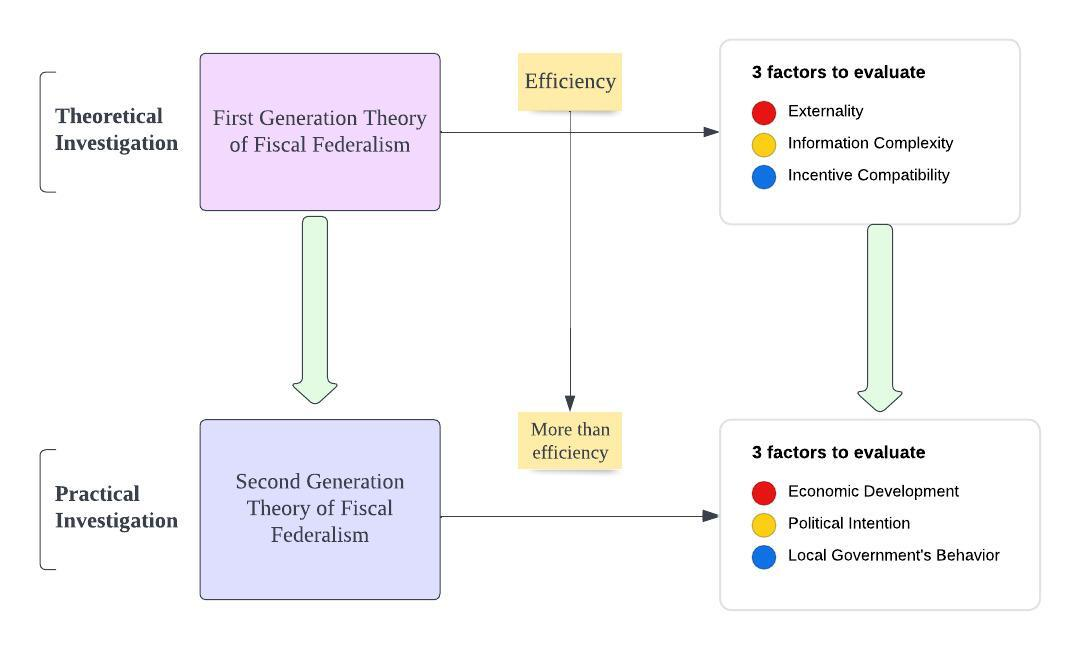
\includegraphics[scale=1]{Chapter-2/Figures/how to evaluate the fiscal federalism.jpeg}
  \caption[How to evaluate the fiscal federalism]{How to evaluate the fiscal federalism
  \texttt{} }
  \label{Figure 2.1}
\end{figure}


To summarize, as is shown in Figure \ref*{Figure 2.1}, initial research about fiscal federalism designed a theoretical ideal framework to supply public goods efficiently. In developed countries especially in America, scholars did find some empirical evidence to support the benefits of this decentralized fiscal structure. However in developing countries, the fiscal federalism didn't work out perfectly, this administrative fact inspired the second-generation theory, scholars starts to focus on the other side of the coin. 

Except for the combination of revenue and responsibilities within each jurisdiction, the interaction between governments is also an intriguing topic for fiscal federalism researchers. The interaction between governments can be divided into horizontal interaction which means the interaction among same level, and vertical interaction which means interaction between central and subnational governments. I'll focus on the vertical interaction in this paper.

\section{How Intergovernmental Transfer Decision is Actually Made}

\subsection{Game Theory Modeling of Bargaining Process}
In America, every year nearly \$700 billion, or nearly 20 percent of overall federal revenues, are allocated toward various state and local government grant programs. The mechanism of intergovernmental transfer distribution has always been an intriguing topic in the public finance area. 

The grants distribution decision in democratic countries is viewed as an bargaining game within a specific decision-making group, such as a specific committee, the congress or the house,depends on which group is the decisive institution. For the bargaining models to simulate the grants distribution bargaining, four assumptions are quite important among all the necessary assumptions: recognition rule, voting rule, amendment rule and money-distribution rule. Recognition rule means how to decide who to make the proposal. In another word, the rule to choose an agenda setter.for example most of the literature assume the random recognition rule \cite{kalandrakis2004three,anesi2015bargaining,diermeier2011legislative,rosenstiel2021congressional}, which means $n$ members among the decision making institution have equal probabilities to be chosen to make the initial proposal. Voting rule means the standard to judge if the proposal is passed,common voting rule include majority rule and unanimously voting rule. Amendment rule means the constraints on making amendments,ranging from the closed rule, in which no amendments are allowed, to the open rule, in which any and all (germane) amendments are allowed. Grants-type rule means how grants could be manipulated by decision making institution, for example, some scholars assume the decision making institution can directly decide the number among the receivers, which is referred as "earmarks" or "pork barrel" spending model.

Baron and Ferejohn \cite{baron1989bargaining} is the fundamental work for all the following bargaining model analysis. They assume random recognition, majority voting rule and earmarks rule. Baron and Ferejohn \cite{baron1989bargaining} and the generalization of their work by Banks and Duggan\cite{banks2006general} show that legislators with proposal or agenda-setting power receive a disproportionate share of funding. Another feature of the equilibrium is that funds only go to legislators that vote for the proposal which is the winning coalition, with zero dollar goes outside of the winning coalition. Besides, according to their inference, when the proposal are brought up under closed rule, the winning coalition is minimal, which means members of the winning coalition maximize their benefits.

Though pioneering in this field, in actual political environment,bare amounts of grants are similar to "earmarks", the earmarks assumptions heavily restrict the explanatory power in grants distribution. Martin \cite{martin2018dividing} extends Baron and Ferejohn's model by loosen the earmark assumption. He restrains the power of members in decision making institution by only allowing them to decide the factor of the formula, not decide the number arbitrarily. As mentioned in Chapter 1, this modification in assumption is a big step to the actual political and administration life. Martin gets some different conclusions compared to Baron and Ferejohn, unlike Baron and Ferejohn’s model, Martin predicts an oversized winning coalitions, and emergence of persistent winning blocs. Besides, he proved that when bargaining over a low-dimensional formula (i.e., a formula based on a small number of state characteristics), legislators have relatively little latitude in targeting funds to specific districts, this prediction is supported by some empirical evidence, Martin studied all the existing formula grants and count the number of the factors in the formula, he points out that 95\% of the formula have less than 5 variables, which means members have less than 5 dimensions to bargain about, the ability to manipulate the formula is highly limited. Since members can only decide the factors among the formula, inevitably, some jurisdiction with similar features can be a free riders, even if the free riders do not belong to winning coalition, thus Martin predicts positive distribution outside the winning coalition. 

\subsection{Some Empirical Evidence for the Grants Distribution}
Except for the general introduction related with intergovernmental transfer in Chapter 1, a challenge with the distribution of IGT is that they take place in a political environments, where individual political agendas have the potential to influence the outcome of IGT allocations in ways that are inconsistent with the intended structure of the distribution procedures.Based on some classic game theory analysis within the congress. Given the important role of GIA in the US federal system, the influence of politics on the allocation of IGT often comes at a high cost. There is plenty of anecdotal examples that illustrates the potential costs, including Robert Carlyle Byrd's spending two decades of his career directing as much federal spending as possible to his home state, saying he wanted to be "West Virginia's billion-dollar industry". 

In Markusen, Saxenian and Weiss's \cite{markusen1981benefits} descriptive study, they define three distinctive swings in the distribution of federal grants to cities in the 1960s and 1970s during which federal grants grew by a tremendous amount and northeastern and midwestern cities benefit most from 1965-1972, southern and western cities benefits most from 1972-1975, and a slight swing back in favor of the first group from 1975-1978. One possible inference in their article is that the political background may partially explained this swings. Stegarescu \cite{stegarescu2006decentralised} explains that the degree of IGT decentralization is a result of population, unemployment, trade-openness, presidential regimes and electoral systems based on the test result of the panel data of 17 nations. Kasdin \cite{kasdin2016decision} does an empirical test and mentions that state or local government governmental network complexity is a factor influencing federal transfer amount and federal controlling extent. He finds that higher-level government tends to relinquish some control when lower governmental network is highly complicated, but the amount of the transfer is negatively related with the complexity. One possible relationship behind this relationship is that high complexity is a barrier hinder politicians to claim the political credit, thus they are less motivated to secure the fiscal revenue for their representative jurisdiction. Larcinese, Rizzo, Testa \cite{larcinese2006allocating} tested the impact of the president on the amount of federal transfer to state government. They find that state that heavily supported the incumbent president in past presidential elections tend to receive more funds. Wallis \cite{wallis1987employment} also emphasizes the political effect on the amount of intergovernmental transfer. He claims that states with the high volatility of presidential vote receive significantly more federal support based on his study on the longitudinal data of all states in the U.S. Markusen, Saxenian and Weiss \cite{markusen1981benefits} defined the supply side and demand side when investigating the mechanism of the IGTs decision-making process, even though they don’t point out the specific factors, they emphasize that the IGTs is the result of the political, economic and social characteristics of both demand and supply side.

All these literature seems imply the political factor even some biased factor impact the intergovernmental transfer. To summarize the literature listed above, one implication is that the factor that impact the intergovernmental transfer comes from not only from the legislative decision-making institution, also from administrative branch. Another implication is that political stance of local jurisdiction seems influential in intergovernmental distribution. 

\section{An Empirical Investigation on IGT Distribution Mechanism}
Combined with Martin's \cite{martin2018dividing} conclusion introduced in section 2.2.1 and all the literature implying the political impact mentioned above, I design and conduct an longitudinal empirical test to statistically investigate the intergovernmental transfer mechanism. Specifically, I try to solve two questions in this empirical design, for one, following Martin's inference, how much extent does states share similar characteristics so the IGT benefits goes outside of the winning coalition. Another questions I wander is, following Markusen, Saxenian and Weiss's framework, if we got the social and economic characteristics control, how much can political factors affect the IGT. The reason I focus on the political factors is that, contradictory to what we discussed in section 2.1, the political factor seems unrelated to efficiency, thus may cause more distortion and waste of resources. Besides, examination on political factors could be important because of the sharp rise in hostility between democratic and republican parties. The potential effects of political party control may impact the IGT grants distribution significantly.  

\subsection{Sample and Characteristic Selection}
I focus on the direct IGT from federal government to state governments in America. To incorporate the political impact into the data framework, I did a stratified sampling to collect states sample from traditional republican states, traditional democratic states and swing states.
The state grouping method are based on two criterion, the historical presidential election result and the winning rate following Beachler,Donald,Bergbower,Matthew etc.'s work \cite{beachler2015presidential}. The democratic states and republican states are those chose same party in the president election since 1984 with wining rate over 58\%. The swing states are those have chosen president from two parties and the winning rates are less than 58\%.

The states collected into my sample can be listed as Table \ref*{Table 2.2}

% Table generated by Excel2LaTeX from sheet 'Sheet1'
\begin{table}[htbp]
  \centering
  \caption{States Sample and Grouping}
    \begin{tabular}{p{7.57em}cc}
    \toprule
    States & \multicolumn{1}{p{7.93em}}{Group} & \multicolumn{1}{p{6.855em}}{Code} \\
    \midrule
    Wyoming & \multicolumn{1}{c}{\multirow{5}[2]{*}{Red States}} & \multirow{5}[2]{*}{0} \\
    Idaho &       &  \\
    Kansas &       &  \\
    Nebraska &       &  \\
    North Dakota &       &  \\
    \midrule
    Maryland & \multicolumn{1}{c}{\multirow{5}[2]{*}{Blue States}} & \multirow{5}[2]{*}{1} \\
    Massachusetts &       &  \\
    Rhode Island &       &  \\
    New York State &       &  \\
    Washington &       &  \\
    \midrule
    Pennsylvania & \multicolumn{1}{c}{\multirow{4}[2]{*}{Swing States}} & \multirow{4}[2]{*}{2} \\
    Nevada &       &  \\
    Wisconsin &       &  \\
    Ohio  &       &  \\
    \bottomrule
    \end{tabular}%
  \label{Table 2.2}%
\end{table}%

 The social and economic characteristics that commonly included in the formula when doing the intergovernmental transfer are population, working age population weight, median household income, unemployment rate and road mileage \cite{dilger2015federal}. I collected all factors mentioned in Dilger's service\cite{dilger2015federal} of the sample states, and did proper operation for data regression convenience and better data visualization. The characteristics I collected and source of data can be listed as Table \ref*{Table 2.3}.

% Table generated by Excel2LaTeX from sheet 'Sheet1'
\begin{table}[H]
  \centering
  \caption{Social characteristics for Sample States}
    \begin{tabular}{cp{6.43em}p{9.285em}p{5.855em}p{5.355em}}
    \toprule
    \multicolumn{1}{p{4em}}{Variables } & Definition & Operation & Source & Time Period \\
    \midrule
    lgp   & \multicolumn{1}{c}{Population } & Log transformation  & Census of bureau & 2000-2019 annually collected \\
    \midrule
    wapw  & Working age population weight & No operation & Census of bureau & 2000-2019 annually collected \\
    \midrule
    mhi   & State median household income & Log transformation  & Census of bureau & 2000-2019 annually collected \\
    \midrule
    ur    & unemployment rate & No operation & Census of bureau & 2000-2019 annually collected \\
    \midrule
    prm   & public road mileage & Log transformation  & Bureau of transportation statistics & 2000-2019 annually collected \\
    \bottomrule
    \end{tabular}%
  \label{Table 2.3}%
\end{table}%

\subsection{Principle Components Analysis of Social and Economic Characteristics}
%%principle components analysis
%%%%%%%%%%%%%%%%%%%%%%%%%%%%%%%%%%%%%%%%%%%%%%%%%%%%%%
As mentioned above, too many factors may exists in the formula that decides the grants distribution. What's even worse, one can distinguish the multicollinearity problem in the variables I collected just by intuition, for example, working age population weight and unemployment rate are strongly related variables, higher population is doomed to occupy more public road. To answer the first question,these two problems are obvious hinder thus it's hard to judge how similar jurisdictions could be in social and economic characteristics directly. So I conduct a primary components analysis to reduce the data dimension and overcome multicollinearity problem to check if the reduced-dimension data are cluster distributed or scattered distributed.

\begin{figure}[H]
  \centering
  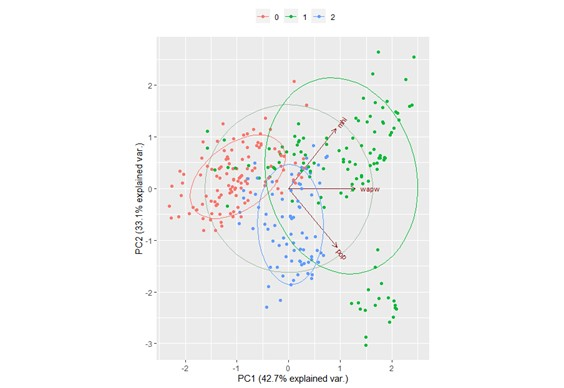
\includegraphics[scale=1]{Chapter-2/Figures/pca.jpg}
  \caption[Social Characteristics Principle components Analysis]{Social Characteristics Principle Component Analysis
  \texttt{} }
  \label{Figure 2.2}
\end{figure}



\subsection{Political Impact Investigation}
%%political factor regression
%%%%%%%%%%%%%%%%%%%%%%%%%%%%%%%%%%
The goal of this section is to  develope and test a theoretical framework that seeks to further advance the understanding of how the above factor outside of the bargaining institution can affect the spatial distribution of IGT. Toward this end, based on the literature implication I collected in section 2.2.1 and 2.2.2, I explore how combination of party control across legislative and administrative branches affects the distribution of IGT. The factor I'm interested includes whether legislative and administrative branches is unified, whether Democratic or Republican party has different preferences, and whether party control is aligned across the federal and state governments.
The general hypothesis proposed is that party control filters into the distribution of IGTs through pressures imposed on administrators from central government officials that are seeking political support in certain states. In addition to party control, we also examine how the perceived importance of a state in the federal political process affects the distribution of IGT. The effects of such pressures becomes visible in several ways, including through party loyalties and that loyalties in the award process who are responsive to. The distribution of IGT is affected by (1) political party distribution across the federal and state government, and by (2) political party affiliation (i.e., Republican or Democratic party). We also examine how the perceived importance of a state in the federal political process affects the distribution of IGT. In addition, to gain insight into we also examine whether a particular state is considered a battle ground state.


\textbf{Hypothesis 1–The unified Government Hypothesis}

Unified government means the administrative branch and legislative branch on federal level coming from same party. Unified government is likely to spend a higher overall spending scale since the financial powers are less limited.

\textbf{Hypothesis 2–Party Specific Hypothesis}

Democratic and republican parties have different preferences on the IGT scale. The preference on IGT of different parties is fuzzy here, since two possible inference may be reasonable here. In terms of the scale of government, the democratic party prefers a big government, which would lead to a higher-scale IGT, and the republican party holds the opposite idea. In terms of the administrative structure, democratic government tends to establish a centralized government, whereas republican government prefers a decentralized structure. In this way, we can get a opposite conclusion

\textbf{Hypothesis 3–Alignment Hypothesis}

The allocation of the IGT are affected by the political ideology. The federal government is likely to allocate more IGT to states that are controlled by same party.

\textbf{Hypothesis 4–Battle Ground States Hypothesis}
The competition level between two parties in state would affect the IGT received by that state government. The federal government is motivated to get elected or reelected; thus, the federal government is willing to put resources and supply more public goods to states that matter a lot for their election to get political credits.




